\documentclass[11pt,letterpaper]{article}
%test2
% \linespread{1.04} % linespread for 10 pt computer modern font
%\linespread{0.901} % linespread for 11 pt computer modern font
%\usepackage{helvet}
%\renewcommand{\familydefault}{\sfdefault}

%XXX: Packages
\usepackage{times}
\usepackage[utf8]{inputenc}
\usepackage[margin=1in]{geometry} % corrects the margins
\usepackage[normalem]{ulem}	                        % underlining!
\usepackage[table,usenames,dvipsnames]{xcolor}      % color
\usepackage{enumitem}                               % [inline]
\usepackage[noadjust]{cite}
\usepackage[compact]{titlesec}
\usepackage{extarrows}
% Math
\usepackage{amsmath,amssymb,amsfonts,amsthm,dsfont} % math
% Figures
\usepackage{graphicx,wrapfig,subcaption}
\usepackage{tabularx}
\usepackage{adjustbox}
%\usepackage[font=footnotesize]{caption}
%*****************************************
% Space Adjustments
\addtolength{\textfloatsep}{-1mm} % reduce space between figs & text
\addtolength{\intextsep}{-1mm}	   % reduce space between intext fig & text
%\addtolength{\floatsep}{-5mm}		 % reduce the space between figures
% \setlength{\belowcaptionskip}{-3pt}
% \setlength{\abovecaptionskip}{3pt}
%*****************************************
% Section formatting
\usepackage{titlesec}
%\titleformat{\section}{\bf\Large}{\thesection}{0.5em}{}%[\titlerule]
%\titleformat{\subsection}[runin]{\large}{\thesubsection.}{0.5em}{}
\titlespacing{\section}{0pt}{*1.5}{*1.5}
\titlespacing{\subsection}{0pt}{*2}{*0.5}
%\titlespacing*{\subsubsection}{0pt}{*2}{*0.5}
%=============================================================
\usepackage[breaklinks=true, colorlinks, bookmarks=true, citecolor=Black, urlcolor=Violet,linkcolor=Black]{hyperref}
\usepackage{todonotes}

% XXX: Commands:
\def\argmin{\mathop{\arg\min}\limits}
\def\argmax{\mathop{\arg\max}\limits}
\newcommand{\longeq}[2]{\xlongequal[\!#2\!]{\!#1\!}}
\newcommand{\prl}[1]{\left(#1\right)}
\newcommand{\brl}[1]{\left[#1\right]}
\newcommand{\crl}[1]{\left\{#1\right\}}
\newcommand{\scaleMathLine}[2][1]{\resizebox{#1\linewidth}{!}{$\displaystyle{#2}$}}
\newcommand{\indicator}{\mathds{1}}
\newcommand{\always}{\square}
\newcommand{\eventually}{\lozenge}
\newcommand{\myparagraph}[1]{\vspace{1ex}\noindent\textbf{#1.}}

% Comments:
\newcommand{\TODO}[1]{{\color{red}#1}}
\newcommand{\XX}[1]{$\clubsuit$\footnote{XX: #1}}
\newcommand{\YY}[1]{$\spadesuit$\footnote{YY: #1}}
\newcommand{\ZZ}[1]{$\heartsuit$\footnote{ZZ: #1}}

% XXX: Environments:
\newtheorem{theorem}{Theorem}
\newtheorem{proposition}{Proposition}
\newtheorem{corollary}{Corollary}
\newtheorem{definition}{Definition}
\newtheorem{assumption}{Assumption}
\newtheorem*{assumption*}{Assumption}
\newtheorem{remark}{Remark}
\newtheorem*{problem*}{Problem}
\newtheorem{problem}{Problem}
\newtheorem{lemma}{Lemma}

\graphicspath{{figures/}}
\usepackage{wrapfig}
\usepackage [english]{babel}
\usepackage [autostyle, english = american]{csquotes}
\MakeOuterQuote{"}

% Titles
\def\thetitle{Online Master of Robotic}

\begin{document}
\begin{center}{\Large\bf {\thetitle}}\end{center}


\section*{Executive Summary}

This document is a proposal for a new {\bf Online Masters of Robotics} (O. M.Rob.)
to be offered by the Jacobs School of Engineering at the University of
California, San Diego. The proposed program seeks to leverage the
faculty and research resources already existing in the various
Engineering departments that take part in the Jacobs School of
Engineering {\bf Contextual Robotics Institute} to offer a world-class
program in robotics at UC San Diego with the following aims:

\begin{enumerate}
\item Offer an Online Masters level degree in robotics that is
  suitable for graduate students from a range of diverse backgrounds
  and disciplines in Science and Engineering;

\item Provide students with current knowledge and practical experience
  in the broad areas of science, engineering and mathematics that
  comprise the rapidly developing field of robotics;

\item Provide a program that covers the broad areas of robotics while
  offering opportunities for in-depth studies in various areas of
  specialization;

\item Prepare students for a professional career in robotics and
  related areas.
\end{enumerate}

Robotics is one of the fastest growing fields of Engineering with a
high demand for skilled, well trained engineers, that is projected to
continue to grow as robotics become part of everyday life at home, at
school, at the government, and in industry. Yet, there are only few
Master programs nationally and internationally that are focused on the
field of robotics. There are at most one Online Masters Program in
robotics.

The proposed program is multidisciplinary and will draw from a myriad
fields of engineering and science, including computer science,
mechanical engineering, artificial intelligence, computer vision,
electrical engineering, control systems, human-robot/computer
interaction, and biomedical engineering, and will be structure around
*foundational*, *breadth* and *depth* requirements, designed to bridge
the knowledge and experience gap between an undergraduate engineering
degree and a successful career in the field of robotics.

We expect our students to become leaders in robotics in
academia, industry and government. At the completion of the program
students will be prepared to work independently and in teams to
accomplish the many tasks necessary to understand, build and operate
complex robotic systems, including mathematical analysis, mechanical
design, electronics, programming, while accounting for the system's
interaction with the physical and human environment.

\newpage

\tableofcontents

\newpage

\begin{center}{\Large\bf {\thetitle}}\end{center}

\section{Introduction}
\label{sec:intro}

\subsection{Aims and Objectives}

The {\bf Online Masters of Robotics} (O. M.Rob.) program proposed in
this document seeks to leverage the faculty and research resources
already existing in the various Engineering departments that take part
in the Jacobs School of Engineering (JSoE) {\bf Contextual Robotics
Institute} (CRI) to offer a world-class online program in robotics
with the following aims:

\begin{enumerate}
\item Offer an online Masters level degree in robotics that is
  suitable for graduate students from a range of diverse backgrounds
  and disciplines in Science and Engineering;

\item Provide students with current knowledge and practical experience
  in the broad areas of science, engineering and mathematics that
  comprise the rapidly developing field of robotics;

\item Provide a program that covers the broad areas of robotics while
  offering opportunities for in-depth studies in various areas of
  specialization;

\item Prepare students for a professional career in robotics and
  related areas.
\end{enumerate}

The program is designed to be online so that we are able to reach a
broad geographic population, and provide educational experience to a
community that until now has been underserved. The rising cost of
higher education, along with the economic challenges faced in
residential education leave behind a large population of students;
many of them are our graduates from years or decades ago, who need to
keep up with changing technological realities. Many of these students
cannot attend residential education at any price due to career
constraints or family obligations. Further, emerging areas, such as
robotics, represent a leading edge of technological advances that
simply cannot be taught by community colleges or our own extension
programs. We anticipate there will be a large demand for this online
Master degree.

Our faculty and courses will come mostly from the Computer Science and
Engineering (CSE), Electrical and Computer Engineering (ECE), and
Mechanical and Aerospace Engineering (MAE) Departments at the JSoE.

One of the main challenges in establishing a successful graduate
program in Robotics is making sure that students coming from diverse
engineering and science fields can fully benefit from the offered
courses and research opportunities regardless of their background. We
expect most of our students to come from undergraduate degrees in
traditional, robotics-related majors such as Mechanical Engineering,
Electrical Engineering, and Computer Science. We also expect a diverse
mix of experiences, from fresh graduates to more seasoned
professionals looking for opportunities of learning and growth in the
ever present field of robotics. We accomplish this goal by
establishing *foundational*, *breadth* and *depth* requirements, to be
discussed later. These requirements are designed to bridge the
knowledge and experience gap between an undergraduate engineering
degree and a successful career in the field of robotics.

The program will draw from many fields of engineering, including
computer science, mechanical engineering, artificial intelligence,
computer vision, electrical engineering, control systems,
human-robot/computer interaction, and biomedical engineering. 

We expect our students to become leaders in robotics in academia,
industry and government. At the completion of the program students
will be prepared to work independently and in teams to accomplish the
many tasks necessary to understand, build and operate complex robotic
systems, including mathematical analysis, mechanical design,
electronics, programming, while accounting for the system's
interaction with the physical and human environment.

The Master of Data Science will be priced at a point that is
comparable to other online professional Masters degrees, for example
those offered in Data Science by Georgia Tech, University of Michigan,
and the University of Illinois, Urbana Champaign.

The formal name of the program, as it appears in the transcript, will
be “Master of Robotics (online)”. The use of the word “online” is
meant to indicate the modality of teaching, in the same way that
transcripts at UC campuses have a special designation for online
courses (at UCSD online courses in the transcript have an “R” at the
end, for example 210R -- other campuses use similar designations). The
use of the word online is not meant to signal a lower quality or rigor
program. The quality and rigor of the online program will be at the
same level as in-person programs. 

\subsection{Historical development of the field}

Robotics is now a 60 year old field. It was initially launched to
provide automation for factories mainly to achieve higher precision
and to alleviate heavy lifts. The objective was to handle dirty, dull,
and dangerous tasks. Around 1970 the field expanded to include service
tasks. The field of robotics today include applications in
manufacturing, services, healthcare, defense and space. Robots are
used in air, ground, space and underwater. Recently, one witness a
trend of increasing integration of robots into the many aspects of
modern society. A few examples include application as diverse as
manufacturing, assistance to elderly people in their homes,
self-driving cars, autonomous aircrafts - drones, exploration of
remote planets, and monitoring of the environment.

While early robots were used entirely on their own and often behind a
fence, modern robots are used in direct collaboration with
humans. Besides a mechanism for physical interaction with the world,
modern robots have a set of sensors that understand the state of robot
as well as the environment in which it operates, and a control system
that regulates the physical interaction with the world based on the
robot's interpretation of the world. Artificial Intelligence (AI) is
used for planning of actions over time and human-robot interaction
methods are used for interoperating with people. Today's robots are
complex systems that require expertise from all areas of MAE, ECE, CSE
and Cognitive Science to be built, programmed and operated.

The field of robotics has grown from a few hundred units per year to
sales that exceeds \$30B/year and is experiencing an annual growth at a
rate of 20\%. This impressive growth rate has been more or less
constant over the last 15 years. As a country, China is seeing 50\%
year-to-year annual growth in sales of robotic systems. India has just
launched a program "Made in India" that is expected to create a similar
growth curve.

The proposed Online M.Rob. program will ready students for working in
this vibrant field of robotics and its impressive and still growing
range of applications. The impact of the program will be felt locally,
as companies such as Qualcomm, General Atomics, Northrop Grumman,
Brain Corporation, TuSimple, and others become more engaged in
robotics, as well as nationally and internationally, as demand for a
skilled workforce in the field of robotics continues to grow. There
are quite a few engineers with a B.Sc. degree that desires to go back
to academia for a M.~Sc. degree but other committments such as family,
mortgage, etc makes a transition for full-time work to full-time
graduate studies a major hurdle. An online degree opens new
opportunities for part-time studies without a need to leave your

\begin{table}[hbtp]
  \centering
  \begin{tabularx}{1.0\linewidth}[c]{ll}
    \hline
    Phase                                & Date         \\
    \hline\hline
    Proposal submitted for UCSD approval & July 2021    \\
    Proposal submitted to CCGA           & Nov 2021     \\
    CCGA Approval (UC Level)             & Jan 2022     \\
    Applications Accepted                & Apr-Jun 2022 \\
    Admission of first cohort            & Aug 2022     \\
    Program Offered                      & Oct 2022     \\
    \hline
  \end{tabularx}
  \caption{Timetable for the development of the program}
  \label{tab:timeline}
\end{table}

The above table shows a timeline of the program approval process. In
the timeline, we will accept applications after CCGA approval. It is
important to realize that since this is a professional Master program,
it can still be successful even if it does not follow the more
traditional December deadline for graduate school applications. We
plan to have two admission cycles per year. Initial enrollments will
start at about 50 students. Over time, we expect enrollments will be
somewhere in the range of 200 - 250 students per year. These targets
will be evaluated continuously as we look at the quality of the
students, the quality of our delivery, and the bandwidth we have for
teaching. For comparison, the fully-online MS in Computer Science at
Georgia Tech has about 6,000 students per year; the Berkeley Master of
Information and Data Science (all online except for a short 3-4 day
on-site immersion) has 600 students per year. Many of the in-person 
M.Sc. program such as UPENN, Utah, OSU have close to 150 admitted students. 
More details on the projected needs will be provided in Section \ref{Sec:ProjectedNeed}.

\subsection{Relationship to existing programs}


There are existing robotics concentrations within ECE and CSE program
that are on-site at UCSD. MAE has a mechatronics specialization which
also has a strong relation to robotics. There is no explicit robotics
degree at UCSD. There are about 160 students in the relevant robotics
specializations. The students coming to UCSD for on-site programs are
pre-dominantly foreign students, that have a strong desire for US
presence as part of the process of getting a job at a US company or a
transfer to a Ph. D. program. Because our proposed online program
would not provide those opportunities (access to job market or
research), we believe it would have a minimal impact on the demand for
the on-site MAE, CSE, and ECE MS programs.

\subsubsection{Impact on enrollments and class sizes of state-supported programs at UCSD​}

As discussed above, the enrollments and class sizes in MS and
undergraduate programs at UCSD will not be affected by the new online
program. In fact, the online program will have a positive impact on
the course offerings in state-supported programs. Indeed, the material
developed for the online program (and possibly even some of the
classes themselves) can be repurposed for state-supported students.

\subsubsection{Interrelationship of the program with programs at other
  UC institutions}

There are no Masters or Ph.D. programs in robotics currently offered
at other UC institutions. There are also no online porgrams in
robotics. On-site programs exising at other institutions will be
discussed in Appendix \ref{App:Comparable}.

There are however, robotics courses offered as areas of concentration
or specialization in various programs in computer science and
engineering, including at UCSD. To name a couple of examples, the
{\bf Robotics and Embedded Software} area of concentration as part of the
M.Eng. Program offered by the Electrical Engineering and in Computer
Science at UC Berkley, the {\bf Dynamic Systems, Controls and Robotics}
area of concentration of the M.Eng. program offered by the Mechanical
Engineering Department at UC Santa Barbara, the ECE Department at UCSD
offers a specialization in {\bf Intelligent Systems, Robotics and
Control}, and the MAE Department offers an specialization in
{\bf Dynamics Systems \& Controls}

We believe that the time is ripe for a graduate degree in Robotics. By
taking advantage of the already existing synergy of teaching in
research taking place as part of the JSoE CRI we aim to establish a
world-class program that can meet the demand for knowledge and
experience in the field of robotics.

The proposed program will offer broader interdisciplinary
opportunities for learning in the area of robotics. The program will
take lessons and curricula from existing classes and adopt them for
online delivery. As mentioned earlier, we believe that it will not
compete with the specializations currently offered at the ECE and MAE
departments.


\subsection{Department or group that will administer the program}

The program will be administered by the JSoE Contextual Robotics
Institute (CRI). 

CRI faculty will be responsible for the academic direction of the program,
including the selection of existing and approval of new proposed
courses. Committees will be staffed and run by CRI faculty. 

Teaching in the program will be done by faculty from MAE, ECE and CSE.
A more detailed governance structure is presented in the section on
Governance (Section \ref{Sec:Governance})

\subsection{Plan for evaluation of the program}

The program will be formally evaluated like all other UCSD graduate
programs, consistent with Senate regulations, every 8 years. This
formal evaluation will include an external review and UCSD graduate
council oversight.

{\bf Learning Outcomes and Metrics}​ Before launch, the program will
define learning outcomes for the entire program and for each course,
and will clearly define how the learning outcomes will be assessed in
each course, and how learning outcomes for each course align with the
learning outcomes for the entire program. The program will work
closely with the UCSD Director of Digital Learning and Teaching +
Learning Commons to develop the learning outcomes, the assessment
plans, and how the collected information will be used to improve the
program.

In addition to the above evaluation of learning outcomes, the program
will also use standard metrics that are part of all program reviews,
including: program size, applicant pool size, admission rate (\% of
applicants offered admission), yield (\% of admitted students who
accept), GPA, graduation rate, time-to-degree, proportion of woman and
URM in the program (i.e.: in the applicant pool, admitted pool, new
student pool, overall student body, and faculty), and post-graduation
placement of students.

The one metric that we want to be careful with is time-to-degree.
While we will definitely collect time-to-degree, it is also important
to realize that in a professional Master program where students might
be balancing several different obligations, time-to-degree is not
always the best indicator of success. Our ultimate goal is to provide
a quality program that works for the schedules of our students, which
means that time-to-degree is less important than for in-person
full-time students.

Another metric that we want to track carefully is completion rate.
Completion rate will be one of the many metrics we will use to assess
the long-term viability of the program. Informed by the metrics of
comparable programs, like Georgia Tech’s online Masters program, and
other online Masters offered by EdX, we expect a completion rate for
the program to be in the 80-85\% range. A drop below 80\% would be a
warning sign. A drop below 60\% would be a red flag, in which case we
will consider drastic remedial measures, and if those do not work, we
will work with UCSD Graduate Council to forge a path forward, possibly
even cancelling the program. We will measure completion rate as the
ratio of the number of students who complete the degree within 5 years
to the number of students who start the degree enrolled at UCSD. This
5-year completion rate will take into account all students, even those
who take a longer time to graduate. This is especially important
because many of the students will be working professionals who might
only be taking one class per quarter, and also juggling other
commitments.

The program will also work with the office of the Chief Information
Officer and with EdX to determine what data can be collected about
online students, and how this data can be used to help increase
student success. The UCSD Chief Information Officer, Vince Kellen, was
hired in 2016, and has a demonstrated track record at prior
institutions of using innovative applications of information
technology in teaching, learning and student success. We look forward
to working with Vince Kellen and his office to ensure the highest
rates of student success in our online program.

{\bf Monitoring and Evaluation}. As mentioned above, the program will
officially be evaluated by the Senate like all other programs, on a
7-8 year period. However, since the start of the program will be the
most critical time, we plan to undergo a formal evaluation of our
program yearly for the first five years with reviews that include: (1)
completion rates for individual classes; (2) completion rates for the
degree program; (3) average time to degree; (4) demographic
information; (5) each statistic in 1-3 broken down by demographic
category; (6) course, TA, and professor response surveys, including
student comments and peer instructor reviews; (7) an evaluation from
Digital Learning in the Teaching+Learning Commons; and (8) financial
data.

The above review cycles will be supplemented by a continuous internal
evaluation process, which, broadly speaking, will include student
feedback \& surveys, teaching evaluations, alumni feedback, and
industry feedback. Based on our experience with the launching of our
Data Science and Engineering MAS and the recent 4-fold growth of the
Computer Science \& Engineering MS, we believe that continuous internal
evaluation, followed up by periodic and deliberate evolution is the
key to success. More specifically, as described in full detail in
Section 2.3.7, we will appoint a Teaching Excellence Coordinator for
the program, a UCSD professor with expertise in online teaching who
will work toward making the program of the highest quality. This
person will continually evaluate student and instructor performance to
understand how to optimize program delivery and student success. We
will intervene when problems arise. Interventions could include:
working with the professor of specific classes to improve course
delivery and assessments; adding additional TA support for classes
where students are struggling; providing additional one-on-one TA and
instructor support for students who are having problems.

{\bf Diversity}. We will pay particular attention to evaluating how our
program performs in terms of diversity, equity and inclusion. However,
defining success for Diversity, Equity, and Inclusion is difficult in
an online program and particularly for an online program in a field
where in-person programs struggle with higher failure rates and lower
retention of students from underrepresented groups (women and URM in
computing). However, we expect online programs to be capable of
reaching a different demographic than our in-person classes, including
students from lower socioeconomic status, working professionals, and
older learners. We will continuously examine demographic data and
student outcomes, by demographic group, to look for areas of concern.
Where there are discrepancies in outcomes by group (e.g., URMs fail at
a higher rate than non URMs), we will compare those outcomes with our
in-person courses and published outcomes from other online programs to
see if the program is doing particularly better or worse by comparison.
Should problems be identified, we will work with the Teaching and
Learning Commons, as well as leverage the large body of research on
inclusive teaching from the education community, to improve these
measures.

To understand how our numbers for diversity, equity and inclusion
compare to the national norms, we will compare our numbers against
both in-person Master programs and prominent online Master programs.

\section{Program}
\subsection{Admission}

The following are the requirements for admission into the online
M.Rob. program:
\begin{enumerate}
\item Students should have a BA/BS in engineering, computer
  science, or a related area, or be able to demonstrate an equivalent
  competency.
\item For acceptance, applicants must have an overall undergraduate GPA of 3.0 on a 4.0 scale
\item Three letters of recommendation
\item Applicants must submit Graduate Record Exam (GRE) general test scores.
\item Test of English as a Foreign Language (TOEFL) scores are
  required for international students whose native language is not
  English.
\end{enumerate}

\subsection{Foreign language}

Foreign language is not required for this degree.

\subsection{Program of study}

There are foundation, breadth, depth, and research and capstone
requirements for the program, as articulated below. These course
requirements are intended to ensure that students are exposed to
\begin{enumerate}
\item fundamental concepts and tools (the foundation requirement), 
\item advanced, up-to-date views in topics outside their area (the breadth 
   requirement), and
\item a deep, current view of their research or
   specialization area (the depth requirements).
 \end{enumerate}
 
Furthermore, students are expected to fulfill a  capstone
requirement as detailed below. The course requirements and how they
are to be articulated are illustrated in Figure \ref{figure}.
	
\begin{figure}[hbtp]
  \centering
  \centerline{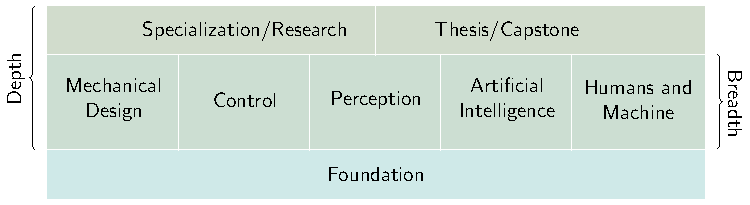
\includegraphics[height=4cm]{diagram}}
  \caption{Sturcture of the program of study}
  \label{figure}
\end{figure}


\subsubsection{Foundation Requirement}

The foundation requirement ensures that master’s students possess the
fundamental concepts and tools from mathematics and engineering
required to fulfill the breadth, depth and research
requirements. Students must complete three graduate courses (twelve
units) to satisfy this requirement. Courses must be taken for a letter
grade and completed with a grade of B- or higher. A list of courses
that can be used to satisfy the foundation requirement is listed below in
the section [Foundation Courses].

The foundation courses provide the basic background needed in the remainder of the program.
\begin{description}
\item[MRO 200R Introduction to Robotics] The course covers fundamental
problems and leading solutions in robot modeling, perception,
planning, and control. Topics are approached primarily from the point
of view of autonomous robot systems -- what and how can we model basic
robots systems, how can the robot perceive the world, and how can it
use that information to move effectively?
\item[MRO 210R Mathemetics for Robotics] This course covers selected topics
in applied mathematics across linear equations, polynomiansl,
non-linear systems, root findings, calculus of variation,
optimization, probability and stochastic processes, etc. To ensure
that students have adequate introduction to applied mathematics for
subsequent courses.
\item[MRO 220R Robot Systems Engineering] The course covers a basic
introduction to the design and implementation of robot systems using
standard tools such as the Robot Operating System, Simulators and
Testing.
\end{description}

\subsubsection{Breadth Requirement}

The breadth requirement ensures that master’s students share knowledge
across broad areas of robotics. Students must complete one graduate
course (twelve units) in three of the five distinct specialization
areas of the program listed above to satisfy this requirement. Courses
must be taken for a letter grade and completed with a grade of B- or
higher. A list of courses that can be used to satisfy the breadth
requirement is listed below in the section \ref{SpecializationCourses}.

\subsubsection{Depth Requirement}

The depth requirement ensures that master’s students acquire expertise
in a general research or specialization area. Students choose a depth
area from one of the five specialization areas of the program listed
above. Students must complete three graduate courses (eight units)
from this list. Courses must be taken for a letter grade. A list of
courses that can be used to satisfy the depth requirement is listed
below in the section \ref{SpecializationCourses}.

Upon approval by the program director, elective courses taken for a
letter grade not listed in the section \ref{SpecializationCourses} may
count toward the depth requirement.

Students will be able to customize their experience in the program by
taking 3 courses in one of the specialization areas. In total at least
nine courses will be available at the launch of the program. 

\subsubsection{Research and Capstone Requirement}

Students must complete the following research and capstone
requirements depending on the chosen plan as discussed below.

Research units are taken on a Satisfactory/Unsatisfactory
basis. Seminar and teaching units may not count toward the breadth,
depth, and research and capstone requirements, although both are
encouraged.

\subsection{Thesis or Comprehensive Exam}

The Online M.Rob. degree can only be pursued under the {\bf
  Comprehensive Examination Plan II}. Plan with the foundation,
breadth, and depth requirements as discussed above. It is possible to
pursue a capstone project as a replacement for the comprehensive exam.

\subsubsection{Capstone (1 course)}

Capstone (1 course) MRO 298R: Capstone Project in Robotics​. This
course consists of a quarter-long project. Students will pick one
project out of several available options, each project from a
different domain. At launch we expect to have projects in: Mechanical
Design, Control, Computing and AI. Over time, we expect to add
additional capstone projects from various disciplines, for example
medical robotics, human robot interaction, robot learning, and
autonomous driving

{\bf Description of capstone element}
The capstone project will consist of one large quarter-long project.
Students will choose from several projects that have been carefully
designed and curated. 

The capstone course will consist of two parts, which will happen
simultaneously. The first part will introduce some background material
in the application domain. The second part will apply techniques
learned throughout the program to a project in the given domain. The
project will cover all topics in the program, including preparing,
storing, analyzing, and visualizing data.

The project will be defined and designed ahead of time. This allows
instructors to create projects that are well thought out from a
pedagogical point of view. These pre-designed projects will need to be
approved by the program director and the Teaching Excellence
Coordinator, to ensure that they meet the course standards.

By default, students will NOT be able to design their own projects.
While individualized projects provide some benefit, including
fostering creativity, it can be hard to ensure a consistently good
selection of projects for hundreds of students.

For each project, there will be one instructor with expertise in the
domain of the project (which we call a “domain instructor”), and
several TAs with expertise in that field. There will also be one
instructor who oversees the entire class, and participates in final
grading (as described below). We call this instructor the “common
instructor”.

{\bf Justification for Pre-designed Projects​.}
As stated in the CCGA handbook, “capstone projects should be
synthetic, tying together two or more areas of specific content that
would typically be the subject of a class or a sequence of classes.”
With this in mind, our goal in the capstone project is to provide a
culminating project in which students apply many aspects of the
material they learned throughout the program in a single project.

We see a tradeoff between pre-designed capstone projects and
customized capstone projects. Pre-designed capstone projects can be
carefully designed and fine-tuned to achieve learning goals, and to
cover a wide gamut of concepts that span the entirety of the program.
However, they rarely provide an open-ended exploration of a topic.
Customized projects do provide an open-ended exploration of a new
topic, but on the other hand, can sometimes fail to meet the learning
goals of the capstone course. This is because each customized project,
by its very nature, is being explored for the first time during the
course, and sometime unexpected obstacles arise that prevent students
from exploring the entire gamut of concepts. As a result, to make sure
customized capstone projects meet learning goals, instructors must
provide a lot of mentoring to the students. With 100 to 150 students
doing capstone projects each year, it becomes all the more difficult
to provide customized projects, while also ensuring that all projects
achieve the learning goals.

In designing our program, we considered the tradeoffs between
pre-designed vs customized capstone, the target size of our program,
our tuition point, and what other online programs do. In the end, we
opted for a default of pre-designed projects. While the projects are
pre-designed, they will still meet the CCGA requirement that the
capstone project ties together concepts from the entire program.
Furthermore, we will also offer students  several ​such pre-designed
projects, to cover of range of possible interests from students.

Finally, as we gain experience in delivering our capstone, we will
also allow a small select set of students, based on grades and
interest, to do a custom project. We envision having at most 10
students a year doing this. Students doing custom projects can work
individually or in groups. Such students would enroll in an honors
version of the capstone course, and would get more individual
mentoring through skype/zoom. The honors version of the course would
be marked as such in the transcript with a different code, for example
“MRO 299R Honors Capstone Project”. Students would apply to
participate in the honors version of the project by proposing a
project in a statement of purpose. The common instructor of the class
will evaluate these statements of purpose and coordinate with possible
instructors and researchers to determine if there is the possibility
of accommodating the project. The common instructor will also make
sure all custom projects are consistent with course standards. For
these custom projects, students will submit their artifact and a
written report. Students in the custom projects will also be required
to do a presentation online. For grading, there will be no automated
grading. The report and presentation will be evaluated by two faculty,
one being a domain instructor (including the possibility of a faculty
advisor), and one being the common instructor, who will have no
relationship with the student. As with all aspects of the program, we
will closely monitor the capstone projects to make sure they meet the
highest standard of quality, and they also meet student needs. If we
find problems, we will make sure to address them immediately.


\subsubsection{Plan II: Comprehensive Examination}

Under this plan, students must execute a special project with an
adviser while enrolled in four units of:

\begin{itemize}
\item MRO 290R. Special Project  (1–12)
\end{itemize}

The student must complete a practical comprehensive examination
designed to evaluate the student’s ability to integrate knowledge and
understanding as well as utilize associated skills. The exam will be
supervised by a faculty committee responsible for the content,
evaluation, and administration of the exam. Each question of the exam
requires the student to produce one or more artifacts representing a
solution. Artifacts may include, but are not limited to, source code,
design documentation, formal reasoning expressed via one or more
proofs or mathematical models, and/or expository prose. Due to the
nature of the exam, with each question taking the form of a project,
the exam will normally be completed over multiple quarters.

\subsubsection{Ensuring Teaching Excellence and Overall Quality of the Program}

To ensure teaching excellence, we will appoint a Teaching Excellence
Coordinator (TEC). The TEC will be a member of the academic senate
whose main responsibility will be to ensure that the program’s
educational quality is of the highest caliber. The TEC will be a
professor with extensive knowledge and expertise in the field of
online education.


\subsection{Residency and Scholarship}

There is no residency requirement for the online degree 

The 40 units of required course work must be taken for a letter grade
(A-F), except for the capstone project (298 course) for which only
Satisfactory/Unsatisfactory (S/U) grades are allowed. Courses for
which a D or F is received may not be counted.

To maintain good academic standing, students must be making timely and
satisfactory progress toward completion of degree requirements and
must maintain a minimum overall GPA of 3.0 at UC San Diego.

\subsection{Faculty advisor}

The program of work shall be under the supervision and subject to the
approval of a member of the faculty of the program.


\section{Projected Need}
\label{Sec:ProjectedNeed}

Market demand for robotics technology has experienced robust growth in
the recent years and is forecast to accelerate even more rapidly as
technologies as diverse as driverless vehicles, artificial
intelligence, and cloud computing gain acceptance and become part of
everyday life. According to \cite{murphy2017}, the robotics marked in
various segments, such as industrial, commercial, military and
entertainment, is expected to grow at a rate of 18\% in the next ten
years. The industrial robotics segment alone, according to \cite{glaser2017},
is forecast to experience three fold growth.

The emergence of robotics as a key component of modern industry offers
enormous opportunity for the professional placement of graduates after
conclusion of the program. Opportunities abound locally, e.g. at
Qualcomm, General Atomics, Spawar, etc, as well as domestically and
internationally. Those opportunities are expected to be the main
driver of demand for the program, offering students from diverse
engineering backgrounds an opportunity to further their knowledge in
the field of robotics at one of the world premier robotics
research institutions.

The program is carefully designed to satisfy the needs of the growing
robotics marketplace while blending practice with theory around the
research interests of the participating faculty. The synergistic
combination of faculty from three departments allows the program to
offer broad coverage of robotics relevant disciplines as well as
opportunities for pursuing in-depth specialization in areas of
interest.

We forecast an initial annual cohort of 50 students that will
eventually grow to 200 by 2025. We anticipate that the students will be
30\% international, 70\% domestic within which 50\% in-state.

Fields such as autonomous driving vehicles, logistics and service
applications are seeing massive annual growth and report that 3 out of
10 positions are unfilled today and growing rapidly.

\section{Faculty}

The following current JSoE faculty is expected to participate in the
program:

\begin{enumerate}
\item Henrik I. Christensen, CSE, Professor, Ph.D.
\item Laurel Riek, CSE, Associate Professor, Ph.D.
\item Ryan Kastner, CSE, Professor, Ph.D.
\item Steven Swanson, CSE, Professor, Ph.D.
\item Sicun Gao, CSE, Assistant Professor, Ph.D.
\item Manmohan Chandrakar, CSE, Assistant Professor, Ph.D.
\item Falko Kuester, SME \& CSE, Professor, Ph.D.
\item Hao Su, CSE, Assistant Professor, Ph.D.
\item Rose Yu, CSE, Assistant Professor, Ph.D.
\item Michael Yip, ECE, Assistant Professor, Ph.D.
\item Nikolay Atanasov, ECE, Assistant Professor, Ph.D.
\item Nuno Vasconcelos, ECE, Professor, Ph.D.
\item Mohan Travedi, ECE, Professor, Ph.D.
\item Xiaolong Wang, ECE, Assistant Professor, Ph.D.
\item Tom Bewley, MAE, Professor, Ph.D. 
\item Jorge Cortes, MAE, Professor, Ph.D. 
\item Sylvia Herbert, MAE, Assistant Professor, Ph.D.
\item Sonia Martinez, MAE, Professor, Ph.D. 
\item Mike Tolley, MAE, Assistant Professor, Ph.D. 
\item Nick Gravish, MAE, Assistant Professor, Ph.D.
\item Tania Morimoto, MAE, Assistant Professor, Ph.D.
\item Mauricio de Oliveira, MAE, Adjunct Professor, Ph.D.
\item Joseph Wang, Nanoengineering, Professor, Ph.D.
\end{enumerate}

The above roster of leading scientists with a diverse set of
expertises in the field of robotics --- as supported by their detailed
CVs to be found on a separated document attached to this proposal,
provides an excellent starting point from which the proposed program
can mature and grow. We anticipate the hiring of additional faculty in
the near future by the JSoE that could be brought to contribute and
complement the above roster.

Please find in the appendix \ref{sec:SupportLetters}, letters from the
chairs of the CSE, ECE, and MAE departments supporting the engagement
of the above listed faculty on the proposed program.

\section{Courses}
\label{sec:courses}
\subsection{Course delivery}

{\bf Instruction}​. All courses will be delivered through a combination
of the edX online platform and the edX Studio hosted at UCSD. The
course content will include:

\begin{itemize}
\item Video lectures​. Video mini-lectures (4-20 minutes) teach
  course content as well as provide live-coding examples which
  encourage students to work through their own code in parallel with
  the instructor. In addition, there are a series of guest lectures
  which introduce students to faculty at UCSD.
\item Readings​. Students
  are given brief readings with either design or course content to
  review.
\item Discussion forum prompts​. Students are prompted
  periodically to engage in discussions regarding course content. They
  are given questions to help facilitate that discussion.
\item  Formative
  quizzes​. Ungraded short practice quizzes allow student to get
  feedback on their learning periodically in the course.
\item  Graded
  quizzes. ​Graded quizzes are short quizzes that are not worth a large
  portion of the grade. Students will not be proctored during these
  quizzes. This mirrors a practice for in-person courses where some
  instructors use online graded quizzes that are not proctored.
\item Projects. Some classes will have project components, which will
  be graded using a variety of approaches, including: (1) automated
  grading (2) TA/Instructor grading (3) peer grading with careful
  rubrics and appealable grades (note that peer grading is also a
  practice that is beginning to gain traction for in-person classes)
\item Exams. ​Exams will be proctored using Software Secure, a leading
  e-proctoring system that verifies student identities and monitors
  students during exams. When an exam starts, Software Secure
  authenticates students using a photo ID through a webcam, and
  requires a room scan of the test environment. During the exam,
  Software Secure monitors and records the learner (through a webcam)
  and computer desktop (using desktop monitoring software) to catch
  any inappropriate physical or online activity. The course team can
  specify the rules (e.g.: no phones, no calculators, no going to
  other websites, etc.). Any suspicious event is reported by the
  Software Secure team to the instructor at UC San Diego to make a
  determination. Each proctored event (audio + video) is recorded and
  can later be replayed to look at problematic cases, thus providing a
  significant level of monitoring. This kind of e-proctoring has
  already been approved by UCSD Graduate Council for graduate R
  (remote) classes.
\end{itemize}

{\bf Office hours:} The instructor and each TA will hold two kinds of
office hours: ​scheduled ​office hours, and ​ad-hoc o​ ffice hours.

Scheduled office​ ​hours ​will happen at advertised times. done either
through online video chatting (using tools like Google hangouts,
Google chat), or through online question forums (where the idea is
that at certain assigned times, there will be someone monitoring
questions non-stop and answering right away) The instructor will use
feedback throughout the class to fine tune the amount of scheduled
office hours, and appropriate times for these office hours (especially
considering the global audience of the program, which includes issues
with time zones) The second kind of office hours will be ​ad-hoc office
hours.​ These will consist of instructors and TAs logging into online
forums periodically to answer questions that have been posted. For
example, each TA might be asked to spend 30 minutes a day answering
questions throughout the day (for example, go online 6 times a day and
answer questions for 5 minutes each time).

{Training TAs}: In addition to taking a department’s required course
such as {\em CSE 599 Teaching Methods in Computer Science}, the instructor
will be responsible for training the TAs to make sure they are
effective in the setting of an online class. This will include making
them familiar with the online platforms, understanding how to answer
questions online, and how to hold online office hours. Even through
the class is online, the instructor and the TAs will meet in person
once a week to manage the class (and of course will coordinate through
email and other online forums more frequently)

{\bf Instructor role}:​ The instructor will monitor forums to make sure
that questions are answered appropriately. In an online setting, the
instructor can also weigh in on questions that have already been
answered. In fact, office hours through an online forum provide much
more oversight than traditional in-person office hours. Indeed, in a
traditional setting, the in-person interactions between a TA and
students are not recorded and not looked at by the instructor. If a TA
answers a question incorrectly (or just not as well as they should
have) during in-person office hours, neither the student nor the
instructor find out about it. However, in an online forum, the
openness and transparency provides oversight not only from the
instructor but from other TAs ​and ​other students, who can also weigh
in on the discussion.

By seeing all the questions that are asked, the instructor can use the
online office hours and online forums to get a good sense of where
student misconceptions are. The instructor can then address these
misconceptions by providing additional content, or additional
assignments. Furthermore, in a online setting, there is also the
potential for a fine-grained assessment of student mis-understandings.
Indeed, because students are progressing in the course online (which
can include practice quizzes to test understanding), the instructor
can look at the rate of progression of students to pinpoint where
students are getting confused. For example, if the instructor notices
that, say question 3 of the test quiz of the second online lecture is
disproportionately answered wrong, the instructor will know that the
concept covered by that question is a source of confusion.

\subsection{Courses}
\label{Sec:ExistingCourses}

\subsubsection{Foundation Courses}
\label{FoundationCourses}

The following courses can be used to satisfy the foundation
requirement:

\subsubsection{Specialization Courses}
\label{SpecializationCourses}

{\bf Mechanical Design}


{\bf Control}


{\bf Perception}


{\bf Artificial Intelligence}

  
{\bf Humans and Machines}


\section{Resource Requirements}
\label{Sec:ResourceRequirements}

We estimate the following resource needs for the first five years in
the categories listed below. Funding to cover these costs will come
primarily from tuition generated by the projected enrollment discussed
earlier in the section [Projected Need].

The proposed program is inline with the current growth plan by the UC
San Diego. 

By taking advantage of the existing alignment of the proposed program
with the participating faculty, there will be minimal reallocation
impact on the contributing M.S. and Ph.D. programs at CSE, ECE and
MAE. 

\subsection{FTE Faculty}

We will offer this program by engaging a number of faculty from
various academic units through a combination of off-load and on-load
teaching. Off-load teaching is done (and paid) in addition to the
regular faculty obligations. This is similar to the way faculty can
get paid for consulting, which is done in addition to their regular
obligations. On-load teaching is done as part of the regular teaching
load, and the academic unit that is contributing the faculty effort
gets reimbursed the full cost of the faculty effort.

On-load versus off-load teaching is an important issue that requires
constant monitoring and adjustments as needed. As a matter of
principle, we are committed to ensuring excellence in instruction,
taught with senate faculty, and with the constraint of not affecting
state-funded programs. The exact ratio of on-load vs off-load is
difficult to predict because of teaching workload variations across
participating units in the program. In some cases, offload teaching
might be the only way to have senate faculty meaningfully participate
in the program without affecting state-supported programs. In other
cases, onload teaching would work perfectly because there is excess
teaching capacity. Adjusting the ratio of on-load vs off-load will be
the key to ensuring that state-supported programs are not affected.
Ultimately, deciding between on-load vs off-load is a resource
management issue that balances all teaching obligations across
different units and different programs, while maximizing participation
by senate faculty.

Having said this, we expect to have 40\% of the teaching done onload
from the start. We will aim for the percent of onload teaching to not
go below 40\%, subject to the constraint of not affecting state-funded
programs. As campus continues to hire more data science faculty, we
will eventually be able to do more teaching onload without
compromising state-funded programs. Finally, ​as will also be explained
later, department revenue will partly be used to fund additional
senate FTEs, which will raise overall teaching capacity (and, thereby,
onload percentage) over time.

We provide some estimates of the money we will pay for various tasks
in the case of offload teaching. These numbers are subject to change,
as we learn more about the work involved in each case.

\begin{itemize}
\item 2 month salary to develop an online class
\item 1/2 month salary to offer an instance of a class
\item 1/2 month salary to do a minor update to a class
\item 1 month salary to do a major update of a class
\end{itemize}

The director of the program is compensated with a 1 month salary. The
teaching execlence coordinator and the academic integrity coordination
each receive a stipend of 1/2 month salary.

Another consideration is advising in state-supported PhD programs: we
believe the online masters program will only have minimal impact on
PhD advising. PhD advising bandwidth can only be affected in the case
of off-load teaching (whereas for on-load teaching, a professor simply
trades one teaching obligation for another, without increasing
teaching load). There are several reasons why we believe the program
will not affect advising bandwidth. First, only a small number of
faculty from any given academic unit will participate in the program
(in CSE, for example, it would be about 4 out of 60 faculty FTEs).
Second, in the steady state, each faculty will only spend a small
amount of off-load time in the program: after the first year or two of
course creation, we anticipate that any faculty doing off-load
teaching will participate at the rate of 1⁄2 month/year in the program
(teaching one course per year), which is a relatively small amount of
faculty time (note: this money can also be thought of as being used
instead of summer salary for faculty who don’t have enough funding to
pay for summer salary). Furthermore, this is not a new precedent:
faculty already spend time and get paid outside of their regular
36teaching/research/service requirements (indeed, these activities,
just like the teaching in the online M. Rob., must be reported in APM
form 025)

Finally, to offset any potential (and small) reduction of faculty
participation in state-supported PhD advising, the profits from the
M.Rob. program will be used to enhance and grow departments as a
whole, including the state-supported programs. This will be a net
positive, as we believe it will largely outweigh any slight reduction
in advising bandwidth. Indeed, the profits will be used toward new
senate faculty FTE, start-up packages, fellowships for all students
(PhD, MS), diversity fellowships, diversity initiatives, and
mentorship programs. Furthermore, a large portion of the expenses of
the program will go to hiring TAs, most of which will be MS students
in a state-funded program, thus making MS programs more enticing (MS
students by default don’t get any funding). In the end, we believe all
these uses of the money to support growth will actually lead to an
overall growth in state-supported PhD programs, and a healthier and
better funded state-supported MS program.

\subsection{Staff}

We will hire one staff member to advise students, advertise the
program, do outreach, help run admissions, and help students with
career planning. We estimate this at about \$100,000 / year.


\subsection{Computing Costs}

Students will need access to cloud computing resources for some data
analysis and machine learning tasks. Based on offerings from the
MicroMasters, we estimate this to be about \$15/course of cloud
computing infrastructure, which will be about \$150 per student going
through the entire program.


\subsection{Teaching Assistants}

For matriculated students, we will aim in the steady state to have one
TA per one hundred students. However, in the first few years, we will
allocate more TAs to make sure that first-time delivery issues are
compensated by good TA support. In particular, we will assume one TA
per 20 students for the first cohort, one TA per 50 students for the
second Cohort, and then one TA per 100 students after that. The TAs
will be expected to run online office hours, answer questions on
forums, update assignments and grading scripts, and run plagiarism
detection tools. 

The Jacobs School of Engineering receives and admits a large number of
MS students each year in the MAE, CSE and ECE departments. Many of
these MS students study central aspects of robotics. Drawing from all
these departments (CSE, ECE, MAE), there is a large pool of potential
TAs for use in the M. Rob. program. In fact, because MS students don’t
typically get research assistantships, they are often eager to get TA
positions. As a result, the TA positions created by the program will
provide well needed support for MS students, and will make
state-supported MS programs more appealing to students.

TAs for the program will be required to take a course on effective
teaching: Such as the CSE 599: Teaching Methods in Computer Science.
The course provides students with guidance on how to best engage
students in discussions and Office Hours, design rubrics, communicate
effectively with students and other instructional staff, effective
pedagogies for teaching, how to assess learning, how to
encourage and enforce Academic Integrity, and how to create an
inclusive environment for a diverse student population. In addition,
we will work with the Director of Online Learning to ensure best
practices in online teaching are taught to TAs in the program.

The cost of a TA is affected by a variety of factors, most importantly
whether the department has to pay for non-resident supplemental
tuition. If a department does not need to pay nonresident
supplemental tuition, a TA costs \$12,557.40 per quarter. If the
department pays nonresident supplemental tuition, the cost is
\$17,591.40. Based on prior statistics, the average cost of a TA is
\$13,211.82 per quarter (the cost is close to the lower end because 
departments does not pay the nonresident supplemental tuition for TAs
who are MS students).

\subsection{Space and Capital Facilities}

There is a need for the Master program to have access to a joint space
for experiential and experimental laboratory based courses. The room
must be able to hold 25 students at a time and be able to accommodate
the projected  load of 75 students per cohort during the program.

\subsection{Other Operating Costs}

Nothing at the moment.

\subsection{Graduate student support}

Since the proposed program is at the Master's level, students
enrolling in the program are expected to cover the costs of tuition,
laboratories and enrollment fees. Such fees are expected to generate
enough revenue to provide adequate instructional support in the form
of teaching assistantships that will be fulfilled primarily by current
Ph.D. students from the CSE, ECE, and MAE departments engaged in
research in the area of robotics with the affiliated faculty.

\subsection{Cost of course development}

We already discussed that faculty will be paid 2 ninths salary (2
months salary) to develop a class. For online classes, there are also
class production costs, which for example include video and studio
production costs. The program will be granted access to the same
institutional infrastructure (in the Digital Learning Hub and
Information Technology Services) that the university is presently
building to support the creation of online courses and degree programs
that advance university priorities. 

\subsection{Revenue to cover costs}

The costs described above will be covered by revenue from the program.
The program charges \$25,000 for the entire program. This academic unit
revenue will cover program expenses like TAs, Instructors and Staff.
Whatever is left over from the academic unit revenue after expenses
are paid will be called academic unit profit.

\section{Graduate Student Support}

\subsection{Financial Accessibility}

The program will provide financially accessible education in multiple ways 

First, the fee structure of the program itself makes the program
affordable. The cost for the entire Master degree is \$25,000. This
price point is significantly lower than typical Master programs, thus
providing an affordable path to a Master degree.

Second, 10\% of the UCSD revenue (before it reaches the academic unit)
will be allocated to financial aid. Some students will be eligible for
financial aid of up to \$5,000, based on financial need.

Finally, it is important to realize that the refund process (and all
aspects of the program) will inevitably be an iterative process. We
will survey students, and understand what issues are causing problems
for our students, and will consider solutions. If there are particular
pain points that affect the welfare of our students, we will
investigate, and address these pain points.

\section{Governance}

The program will be administered by the CRI.

CRI faculty is responsible for the academic direction of the program,
including the selection of existing and approval of new proposed
courses. Committees will be staffed and run by CRI faculty.

The program will be governed by the following administrative structure:
\begin{description}
\item[Program Director​] The director will be a member of the academic
  senate who will ultimately be responsible for the delivery of the
  program, and its ongoing evolution. For the first three years, the
  program director will report to the director of CRI and the chairs
  of CSE, ECE and MAE. After three years, this governance structure
  will be reassessed and updated as needed.
  
\item[Teaching Excellence Coordinator​] Because maintaining quality of
  education is such an important consideration, a Teaching Excellence
  Coordinator (TEC) will be appointed. The TEC will be a member of the
  academic senate whose main responsibility will be to ensure that the
  program’s educational quality is of the highest caliber. The
  responsibilities of the TEC are detailed in Section [ref]. The TEC
  will report to the program director.

\item[Academic Integrity Coordinator]​ Because we want to enforce the
  highest level of academic integrity, an Academic Integrity
  Coordinator (AIC) will be appointed. The AIC will be a UCSD
  professor whose main role will be to ensure that all courses follow
  the guidelines set forth in Section, including running
  plagiarism detection software, and reporting all allegations of
  academic integrity violations. If needed, the efforts of the AIC
  will be supplemented with staff support, for example, to
  organize/manage/follow-up on all allegations of academic integrity
  violation.

\item[Admissions Committee]​ The admissions committee will consist of
   several Senate faculty members appointed by the program director.
   The admissions committee will decide which students are admitted
   into the program.

\item[Support Staff]​ The program will hire a staff member to run the
   following aspects of the program: admissions, academic and career
   advising, financial management, outreach. The staff will report
   to the program director.
 \end{description}
 
\section{Changes in Senate Regulations}

No changes in senate regulations are required.


\appendix
~
\newpage

\noindent Optional Appendices

\section{Complete CVs for principal faculty}

\newpage

\section{Supporting Letters}
\label{App:SupportingLetters}


\subsection{CSE Department Chair}

\subsection{ECE Department Chair}

\subsection{MAE Department Chair}

\newpage

\section{Comparable degree programs}
\label{App:Comparable}

Programs which are comparable to the one proposed here exist in
institutions other than the University of California. The programs
listed below seem to be the closest in scope to this
proposal. Detailed information of these programs can be found on the
provided links. They all pay attention to the multidisciplinary nature
of the field of robotics and involve faculty from multiple departments
and disciplines.

\begin{itemize}
\item The University of Utah \href{}{URL}
\item Carnegie Mellon University
  \href{https://www.ri.cmu.edu/education/academic-programs/master-of-science-robotics/}{URL}
\item University of Pennsylvania
  \href{https://gradadm.seas.upenn.edu/masters/robotics/}{URL}
\item Worcester Polytechnic Institute
  \href{https://www.wpi.edu/academics/study/robotics-engineering-ms}{URL}
\item Orogon State University \href{}{URL} 
\end{itemize}

\newpage

\section{Bylaws}
\label{App:Bylaws}

See attached document.

\newpage

\section{Courses Syllabus}
\label{App:Courses}

**TO BE REVISED**

\subsection{CSE Courses}

**CSE 252A. Computer Vision I (4)** Comprehensive introduction to
computer vision providing broad coverage including low-level vision
(image formation, photometry, color, image feature detection), inferring
3-D properties from images (shape-from shading, stereo vision, motion
interpretation) and object recognition. Companion to CSE 252B covering
complementary topics. ***Prerequisites:*** Math 10D and Math 20A–F or
equivalent.

**CSE 252B. Computer Vision II (4)** Comprehensive introduction to
computer vision providing focused coverage of multiview geometry,
structure from motion, image segmentation, motion segmentation, texture
analysis and recognition, object detection, and image-based rendering.
Companion to CSE 252A covering complementary topics.
***Prerequisites:*** Math 10D and Math 20A–F or equivalent.

**CSE 252C. Selected Topics in Vision and Learning (1–4)** Selected
topics in computer vision and statistical pattern recognition, with an
emphasis on recent developments. Possible topics include: grouping and
segmentation, object recognition and tracking, multiple view geometry,
kernel-based methods, dimensionality reduction, and mixture models.
***Prerequisites:*** CSE 252 or equivalent and CSE 250B or equivalent.

**CSE 253. Neural Networks for Pattern Recognition (4)** Probability
density estimation, perceptrons, multilayer neural networks, radial
basis function networks, support vector machines, error functions, data
preprocessing. Possible topics include unsupervised learning methods,
recurrent networks, and mathematical learning theory. Recommended
preparation: CSE 250B or equivalent. ***Prerequisites:*** graduate
standing.

**CSE 254. Statistical Learning (4)** Learning algorithms based on
statistics. Possible topics include minimum-variance unbiased
estimators, maximum likelihood estimation, likelihood ratio tests,
resampling methods, linear logistic regression, feature selection,
regularization, dimensionality reduction, manifold detection. An
upper-division undergraduate course on probability and statistics such
as Math 183 or 186, or any graduate course on statistics, pattern
recognition, or machine learning is recommended. ***Prerequisites:***
graduate standing.

**CSE 257. Search and Optimization (4)** The course will cover core
algorithms for sequential decision making with an emphasis on their
applications in planning and control problems for autonomous
systems. Topics include: A\* search, rapidly-exploring random trees,
bandit problems and Monte Carlo tree search, deep reinforcement
learning, nonlinear optimization, mixed-integer optimization, and
stochastic optimization. ***Prerequisites:***
graduate standing.

**CSE 276A. Introduction to Robotics (4)** This course provides an
introduction to the fundamentals of robotics across kinematics, sensor
systems, estimation, control, and planning. The contents include
introduction to robotics in general, kinematics of robot systems, robot
arm systems, sensors for robots, basic vision for robots, estimation
methods, perception, robot localization and navigation, control of robot
systems, robot motion planning, robot task planning, robot
architectures, and evaluation of robot systems. It is expected that
students have a solid understanding of linear algebra, can program in
Python or C++, and have a basic understanding of methods for reasoning
under uncertainty. ***Prerequisites:*** graduate standing.

**CSE 276B. Human Robot Interaction (4)** Robots are entering human
spaces. How do we make them functional, useful, and acceptable? This
course explores the core computational, engineering, and experimental
challenges in human-robot interaction. Course topics include shared
autonomy, perception of people and context, coordination, collaboration,
human-guided learning, robot design, and experimental robotics. Students
will review seminal and recent papers in the field and engage in
team-based projects with physical, mobile robots. This class requires
expertise in software development. Prior exposure to robotics, computer
vision, or machine learning is recommended. Students should be
comfortable reading and analyzing scientific papers at the graduate
level. Students may not receive credit for CSE 276B and CSE 291 (A00)
taught winter 2017 with the same subtitle. ***Prerequisites:*** graduate
standing.

**CSE 276C. Mathematics for Robotics (4)** The course will provide a
comprehensive introduction to the key mathematical concepts used for
modeling, implementing, and evaluation of robot systems. The course will
use small home assignments tasks and a larger robot project to exercise
the topics covered in class. The students should have a basic knowledge
of mathematics and know one or more programming languages such as Python
or Matlab for completion of homework assignments. ***Prerequisites:***
graduate standing.

**CSE 276D. Healthcare Robotics (4)** Robotics has the potential to
improve well-being for millions of people, support care givers, and aid
the clinical workforce. This course brings together engineers,
clinicians, and end-users to explore this exciting new field. It is
project-based, interactive, and hands on, and involves working closely
with stakeholders to develop prototypes that solve real-world problems.
Students will explore the latest research in healthcare robotics,
human-robot teaming, and health design. JSoE students should be
comfortable building and experimenting within their area of expertise
(e.g., CSE, software development, MAE, rapid prototyping). Students with
clinical backgrounds should be familiar with translational research
methods. Students may not receive credit for CSE 276D and CSE 291 (H00)
taught spring 2017 with the same subtitle. Program or materials fees may
apply. ***Prerequisites:*** graduate standing.

\subsection{ECE Courses}

**ECE 208. Computational Evolutionary Biology (4)** Evolutionary
biology (e.g., the study of the tree of life) uses computational
methods from statistics and machine learning. We cover methods of
broad use in many fields and apply them to biology, focusing on
scalability to big genomic data. Topics include dynamic programming,
continuous time Markov models, hidden Markov models, statistical
inference of phylogenies, sequence alignment, uncertainty (e.g.,
bootstrapping), and heterogeneity (e.g., phylogenetic mixture
models). ***Prerequisites:*** graduate standing.

**ECE 227. Big Network Data (4)** A course on network science driven
by data analysis. The class will focus on both theoretical and
empirical analysis performed on real data, including technological
networks, social networks, information networks, biological networks,
economic networks, and financial networks. Students will be exposed to
a number of state-of-the-art software libraries for network data
analysis and visualization via the Python notebook
environment. Previous Python programming experience
recommended. ***Prerequisites:*** graduate standing.

**ECE 228. Machine Learning for Physical Applications (4)**
Machine learning has received enormous interest. To learn from data we
use probability theory, which has been a mainstay of statistics and
engineering for centuries. The class will focus on implementations for
physical problems. Topics: Gaussian probabilities, linear models for
regression, linear models for classification, neural networks, kernel
methods, support vector machines, graphical models, mixture models,
sampling methods, and sequential estimation. ***Prerequisites:***
graduate standing.

**ECE 276A. Sensing and Estimation in Robotics (4)** This course covers
the mathematical fundamentals of Bayesian filtering and their
application to sensing and estimation in mobile robotics. Topics include
maximum likelihood estimation (MLE), expectation maximization (EM),
Gaussian and particle filters, simultaneous localization and mapping
(SLAM), visual features and optical flow, and hidden Markov models
(HMM). ***Prerequisites:*** graduate standing.

**ECE 276B. Planning and Learning in Robotics (4)** This course covers
optimal control and reinforcement learning fundamentals and their
application to planning and decision-making in mobile robotics. Topics
include Markov decision processes (MDP), Pontryagin’s maximum principle,
linear quadratic regulation (LQR), deterministic planning, value and
policy iteration, and policy gradient methods. **Prerequisites:** ECE
276A; graduate standing.

**ECE 276C. Robot Reinforcement Learning (4)** Course participants will
explore new methods for robotics, particularly toward enabling robot
manipulators in complex environments. This course is structured to
rapidly consider the previous techniques in robot manipulation to date
and explore methods in reinforcement learning to solve open problems in
robot manipulation. Topics will review kinematics, dynamics, low-level
control and motion planning, and machine learning approaches.
***Prerequisites:*** ECE 276A; graduate standing.

\subsection{MAE Courses}

**MAE 200. Controls (4)** This course covers topics in probability and
stochastic processes, linear control and estimation including optimal
linear control, nonlinear stabilization, and optimal control and
estimation for nonlinear systems. ***Prerequisites:*** non-graduate
students may enroll with consent of instructor.

**MAE 204. Robotics (4)** This course covers topics in robotics,
dynamics, kinematics, mechatronics, control, locomotion, and
manipulation. ***Prerequisites:*** non-graduate students may enroll with
consent of instructor.

**MAE 207. Haptics Interfaces (4)** This course provides an
introduction to the design and control of haptic systems, which
provide touch feedback to human users interacting with virtual
environments and teleoperated robots. Topics include haptic-focused
mechatronic design, system modeling and analysis (kinematics and
dynamics), human-in-the-loop feedback control, and haptic feedback
evaluation. Coursework includes lab-based homework assignments and a
substantial, research-oriented project. This course is directed toward
graduate students and advanced undergraduates in engineering and
computer science. Recommended experience with: dynamic systems,
programming, feedback control design, mechatronics, and hardware
prototyping. ***Prerequisite:*** consent of instructor.

**MAE 207. Bioinspired mobile robotics (4)** Animals are capable of
wonderful feats of locomotion and many of the most cutting edge robots
seek to embody those capabilities. Roboticists have long looked to
nature for inspiration in robot design, actuation, and control. In
this class we will explore the world of bio-inspired mobile robotics
using lecture and project based work. The primary goal of the class is
to expose students to state-of-the-art bioinspired robot platforms,
robot technologies (actuators, sensors, controls), and robot design
principles. This will be motivated and contextualized throughout the
course by examples from biological locomotion.  This course focuses on
locomotion and so we will be keenly interested in mechanics, dynamics,
and control of movement. In this course we will cover varied types of
mobility in robotics and biology including legged locomotion
(running/climbing), flight (flapping wing, fixed wing), continuum
“snake-like” movement (serpentine, sidewinding, rectilinear waves),
and swimming. In order to develop technical skills in robot design
student groups will work on a hands-on research project to design and
test legged robot modules. By the end of this course students will
have gained hands-on experience with experimental robot hardware,
motivated by theory and experiments from
biomechanics. ***Prerequisite:*** consent of instructor.

**MAE 207. Topics in Engineering Science (4)** A course to be
given at the discretion of the faculty in which topics of current
interest in engineering will be presented. ***Prerequisite:*** consent of
instructor.
 
**MAE 242. Robot Motion Planning (4)** Modeling, solving, and analyzing
planning problems for single robots or agents. Configuration space for
motion planning, sampling-based motion planning, combinatorial motion
planning, feedback motion planning, differential models, and
nonholonomic constraints. Basic decision-theory and dynamic programming,
sensor and information spaces.

**MAE 247. Cooperative Control of Multi-agent Systems (4)** Tools for
the design of cooperative control strategies for multi-agent systems are
presented. Topics include continuous and discrete-time evolution models,
proximity graphs, performance measures, invariance principles, and
coordination algorithms for rendezvous, deployment, flocking, formation
of autonomous vehicles and consensus.

\subsection{Other Courses}

**NANO 244. Nanomachines and Nanorobots (4)** The structure and
operational principles of different nature biomotors will be
discussed. Related bio-inspired efforts aimed at developing artificial
nanomotors will also be covered, along with the prospects of using
biomotors and synthetic nanomotors in engineering
environments. ***Prerequisites:*** consent of instructor.

**SE 207. 3D Printable Robotics (4)** 3D Printable Robotics is
studying the design, modeling, simulation, 3D printing and testing of
integrated robotic systems., This has been offered for the past four
years and drawn a nice interdisciplinary student cohort from within
JSoE.

**SE 207. Engineering Human Frontiers (4)** Engineering Human
Frontiers is studying means to augment and recapture human abilities
through a broad range of “prosthetics”.

% Bibliography
%==================================================================%
\bibliographystyle{IEEEtran}
\bibliography{references}
%==================================================================%
\end{document}


